\part{Metodologia}

\chapter{Metodologia}

\section{Fluxo de atividades}

A sequência de atividades que engloba este trabalho baseia-se no modelo CRISP-DM, uma abreviação de CRoss Industry Standard Process for Data Mining (Processo Padrão de Vários Segmentos de Mercados para Mineração de Dados). Este é um modelo de processo e metodologia da IBM que busca orientar os esforços da organização descrevendo as fases típicas e tarefas envolvidas do ciclo de vida em um projeto de mineração de dados \cite{crispdm}. 

A figura abaixo mostra o fluxograma padrão que representa uma visão geral das fases do CRISP-DM.

\begin{figure}[!htb]
    \center{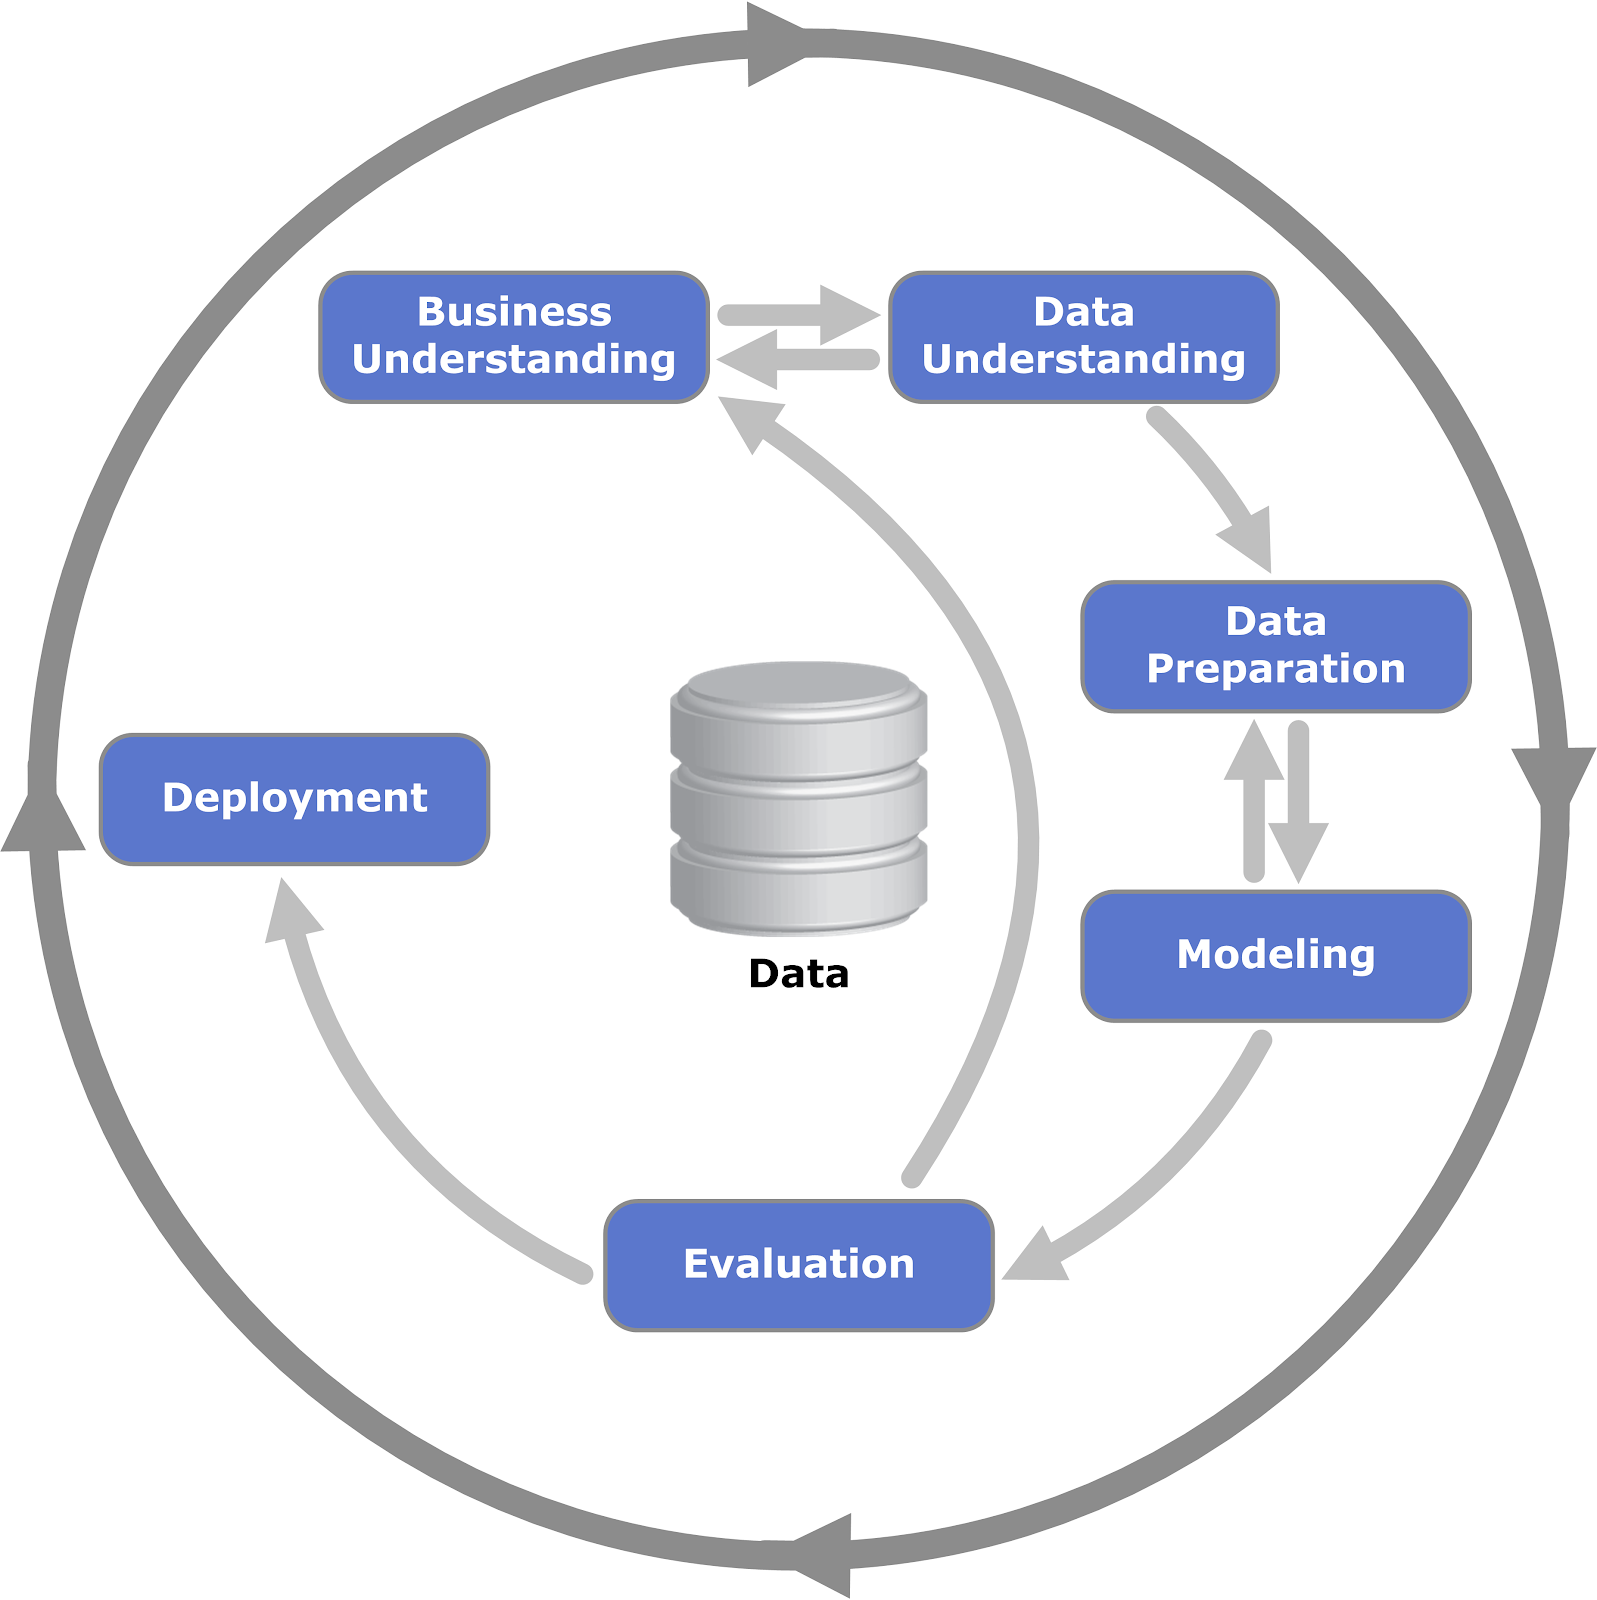
\includegraphics[scale=0.2]
    {figuras/fluxograma_crisp.png}}
    \caption{\label{fig:jupyter} O ciclo de vida da mineração de dados.}
\end{figure}

O modelo CRISP-DM é bastante flexível, podendo ser customizado de acordo com as necessidades do projeto ou da organização. Segue abaixo uma breve descrição das fases ilustradas no modelo.

\begin{itemize}
    \item \textbf{Business Understanding} - Entendimento de Negócios: Trata-se da fase inicial do projeto, onde se investiga as metas de negócios da organização, reúne-se informações básicas e define critérios para o sucesso.
    \item \textbf{Data Understanding} - Entendimento dos Dados: Etapa de verificação dos dados disponíveis a fim de evitar problemas posteriores. Normalmente, esta é a etapa mais longa de um projeto (IBM, 2015), porém, no atual projeto, onde são utilizados apenas textos e labels, não há uma complexidade muito grande na execução desta fase. Mais detalhes sobre o dataset em \textbf{X}.
    \item \textbf{Data Preparation} - Preparação de Dados: “Estima-se que a preparação de dados normalmente consome 50-70\% do tempo e esforço do projeto”(IBM, 2015, p. 19). Como não havia a necessidade de derivar novos atributos, mesclar registros, ou remover registros inválidos, nesta etapa, foram utilizadas técnicas de limpeza de texto e processamento de linguagem natural, como stemização e remoção de stop words. Mais detalhes sobre as técnicas utilizadas em \textbf{X}.
    \item \textbf{Modeling} - Modelando: Nesta fase, a natureza do problema e das metas definidas no Entendimento de Negócios e os dados disponíveis definem as técnicas de modelagem a serem utilizadas. No contexto de classificação de texto com um conjunto já rotulado, opta-se pelo uso de algoritmos de classificação, de aprendizado supervisionado. Estima-se que esta etapa seja realizada em várias iterações. Primeiramente, com os hiperparâmetros padrão e, nas iterações seguintes, refinando-os a fim de buscar por resultados cada vez mais satisfatórios.
    \item \textbf{Evaluation} - Avaliação: Fase onde se analisa e faz inferências sobre os esforços realizado. Para que seja possível cumprir esta etapa de forma objetiva, critérios de avaliação são estabelecidos para os modelos. As métricas são coletadas e analisadas a fim de encontrar e/ou rankear os modelos que melhor atendem aos objetivos do projeto.
    \item \textbf{Deployment} - Implantação: Fase em que serão realizados estudos sobre a arquitetura da plataforma EJ, onde o classificador será implantado, levando em consideração que o modelo será constantemente retroalimentado, visando seu aperfeiçoamento com dados de situações mais próximas ao contexto da plataforma. Para se chegar à esta fase, é necessário repetir o ciclo até o ponto de avaliação ao menos uma vez, de modo que o sistema satisfaça os requisitos do projeto. Esta fase também envolve planejar e monitorar a implementação dos resultados, além de uma revisão do projeto.
\end{itemize}

\section{Experimentos}

Esta etapa do trabalho configura a fase de Modeling do CRISP-DM. Nela, foram utilizados seis diferentes modelos de classificação, sendo eles: SVM, Random Forest, Multinomial Naive Bayes, Decision Tree, MLP e SVC. Todos os modelos passaram pelo processo descrito abaixo, para que, por fim, eles pudessem ser avaliados a partir das métricas obtidas em cada fase de teste utilizando os critérios de avaliação definidos anteriormente.

\begin{itemize}
    \item \textbf{Testar classificador (fase 1)}: trata-se da primeira bateria de testes do classificador, utilizando a técnica de validação cruzada (k-fold cross validation) visando reduzir os efeitos da divisão do conjunto de dados entre teste e treino (mais detalhes sobre esta técnica na seção X). O objetivo desta fase inicial é obter métricas do classificador antes da utilização das técnicas processamento de linguagem natural citadas no capítulo 2, garantindo, assim, parâmetros de comparação para avaliar os efeitos das técnicas utilizadas. 
    \item \textbf{Realizar limpeza do dataset}: aplicação das técnicas descritas no capítulo 2 e 3.
    \item \textbf{Testar classificador (fase 2)}: segunda bateria de testes. Utiliza-se o mesmo Pipeline que foi construído na fase 1, alterando, apenas, o conjunto de dados que agora fora submetido à limpeza.
    \item \textbf{Refinar hiperparâmetros}: utilizando uma técnica otimização de hiperparâmetros, o Grid Search (explicado no capítulo 3), busca-se por parâmetros mais adequados para o atual modelo.
    \item \textbf{Testar classificador (fase 3)}: com os hiperparâmetros encontrados na fase anterior, realiza-se a bateria de testes final.
\end{itemize}

\section{Critérios de avaliação}

A fim de determinar quais métricas devem ser levadas em consideração ao avaliar os modelos de classificação, é necessário ter um entendimento do problema e de como métricas em questão são geradas. No contexto de uma classificação binária, as métricas derivam-se dos conceitos apresentados na matriz de confusão do quadro a seguir.

\begin{table}[H]
\begin{tabular}{|
>{\columncolor[HTML]{93C47D}}l |
>{\columncolor[HTML]{E06666}}l |}
\hline
\begin{tabular}[c]{@{}l@{}}TP - True Positive (Verdadeiro Positivo)\\ Elemento corretamente acusado pelo\\ algoritmo como discurso de ódio.\end{tabular} & \begin{tabular}[c]{@{}l@{}}FP - False Positive (Falso Positivo)\\ Elemento erroneamente acusado pelo \\ algoritmo como discurso de ódio.\end{tabular} \\ \hline
\cellcolor[HTML]{E06666}\begin{tabular}[c]{@{}l@{}}FN - False Negative (Falso Negativo)\\ Elemento erroneamente negado pelo \\ algoritmo como discurso de ódio.\end{tabular} & \cellcolor[HTML]{93C47D}\begin{tabular}[c]{@{}l@{}}TN - True Negative (Verdadeiro Negativo)\\ Elemento corretamente negado \\ pelo algoritmo como discurso de ódio.\end{tabular} \\ \hline
\end{tabular}
\caption{Matriz de confusão para a classe 1 - Discurso de ódio}
\label{tab:confusion-matrix}
\end{table}

Observando a matriz de confusão no \ref{tab:confusion-matrix}, torna-se evidente que os eventos representados de vermelho são indesejáveis, pois representam erros. Contudo, deve-se avaliar o impacto dos dois erros e definir os custos de ambos, e, dessa forma, apontar o mais indesejável. Esta análise serve de base na definição de qual métrica será utilizada na avaliação de desempenho dos algoritmos. Isso porque o algoritmo pode ser tendencioso à realização de determinada classificação, podendo ser benéfico para uma métrica, mas maléfico para outra, tornando imprescindível o uso de múltiplas métricas para tornar a avaliação mais balanceada.
A biblioteca scikit-learn oferece uma série de métodos que retornam métricas e nos ajudam a fazer esta análise. O método “classification\_report”, utilizado neste trabalho, retorna as principais métricas no seguinte formato:

\begin{figure}[!htb]
    \center{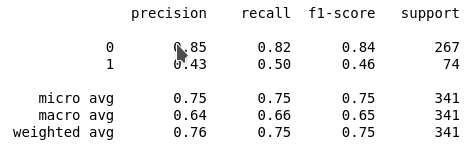
\includegraphics[scale=1]
    {figuras/prs_random_forest.png}}
    \caption{\label{fig:jupyter} Precision, Recall e Score do algoritmo Random Forest.}
\end{figure}

 A precisão, dada como $\rho$, é definada da seguinte forma:
 
 $$ \rho=\frac{\alpha}{(\alpha+\beta)} $$

Onde $\alpha$ são os verdadeiros positivos (TP), e $\beta$ os falsos positivos (FP).

A cobertura ($\tau$) pode ser definida de modo semelhante:

$$ \tau = \frac{\alpha}{(\alpha+\gamma)}$$

Onde $\gamma$ são os Falsos negativos (FN).

Por fim, o valor F1, $\Delta$, é definido pela equação:

$$\Delta = \Bigg(\frac{(\tau^{-1} + \rho^{-1})}{2}\Bigg)^{-1} =2*\Bigg(\frac{\rho\tau}{\rho+\tau}\Bigg)$$

Considerando o contexto do EJ, e que este trabalho almeja apontar comentários com discurso de ódio para serem avaliados por um moderador posteriormente, o custo de permitir que um comentário indevido seja exibido na plataforma é muito mais alto do que o deste comentário ser enviado para a moderação. Sendo assim, a principal métrica para as nossas avaliações dos modelos será o \textbf{recall da classe 1} (discurso de ódio), que penaliza justamente as classificações errôneas, onde um comentário contendo discurso de ódio é classificado como discurso comum.
As métricas micro avg, macro avg e weighted avg representam valores que englobam todas as classes. Para 2 classes, são representadas pelas seguintes fórmulas, onde 0 e 1 são referentes às classes:


$$ 
\rho_{micro} = 
\frac{(\alpha_0+\alpha_1)}{\alpha_0+\alpha_1+\beta_0+\beta_1} 
$$

$$ 
\tau_{micro} = 
\frac{(\alpha_0+\alpha_1)}{\alpha_0+\alpha_1+\gamma_0+\gamma_1} 
$$

$$ 
\rho_{macro} = 
\frac{(\rho_0+\rho_1)}{2} 
$$

$$ 
\tau_{macro} = 
\frac{(\tau_0+\tau_1)}{2} 
$$

$$ 
\rho_{weighted} = 
\frac{(\rho_0+\chi_0)+(\rho_1+\chi_1)}{\chi_0+\chi_1} 
$$

$$ 
\rho_{weighted} = 
\frac{(\rho_0+\chi_0)+(\rho_1+\chi_1)}{\chi_0+\chi_1} 
$$

$$ 
\tau_{weighted} = 
\frac{(\tau_0+\chi_0)+(\tau_1+\chi_1)}{\chi_0+\chi_1} 
$$

Onde $\chi_0$  e $\chi_1$ são a amostra das classes 0 e 1, respectivamente.

Sendo assim, é possível notar que todas essas métricas possuem um certo grau de importância. Para não escolhermos um algoritmo totalmente enviesado para o duscurso de ódio (classe 1) - o que poderia resultar em uma quantidade excessiva de textos comuns (classe 0) sendo enviados para a moderação - decidimos também destacar a métrica macro avg da precisão, que, apesar de ser enviesada para o discurso de ódio (já que ela ignora o fato de possuir menos discursos de ódio), ela engloba ambas as classes, diferente da métrica recall 1.